\documentclass[a4paper,oneside,12pt]{extreport}

\usepackage{mmap}
\usepackage[T2A]{fontenc}
\usepackage[utf8]{inputenc}
\usepackage[english,russian]{babel}


% Текст отчёта следует печатать, соблюдая следующие размеры полей:
% левое — 30 мм, правое — 15 мм, верхнее и нижнее — 20 мм.
\usepackage[left=20mm, right=15mm, top=15mm, bottom=15mm]{geometry}

% \setlength{\parindent}{1.25cm} % Абзацный отступ

\usepackage{setspace}
%\onehalfspacing % Полуторный интервал

\frenchspacing % Равномерные пробелы
\usepackage{indentfirst} % Красная строка

\usepackage{microtype}
\sloppy

\usepackage{titlesec}
\titlespacing*{\chapter}{0pt}{-30pt}{8pt}
\titlespacing*{\section}{\parindent}{*4}{*4}
\titlespacing*{\subsection}{\parindent}{*4}{*4}
\titleformat{\chapter}{\LARGE\bfseries}{\thechapter}{20pt}{\LARGE\bfseries}
\titleformat{\section}{\Large\bfseries}{\thesection}{40pt}{\Large\bfseries}

\usepackage{graphicx}
\usepackage{caption}

\usepackage[unicode,pdftex]{hyperref}
\hypersetup{hidelinks}

%% title begin
\usepackage{wrapfig}

\makeatletter
	\def\vhrulefill#1{\leavevmode\leaders\hrule\@height#1\hfill \kern\z@}
\makeatother
%% title end

%% begin code
\usepackage{listings}
\usepackage{xcolor}

\lstset{
	basicstyle=\footnotesize\ttfamily,
	breakatwhitespace=true,
	breaklines=true,
	commentstyle=\color{gray},
	frame=single,
	keywordstyle=\color{blue},
	stringstyle=\color{red},
	tabsize=8
}

\lstdefinestyle{lispinline}{
	frame=none,
	language=Lisp
}

\newcommand{\code}[1]{\texttt{#1}}
%% end code

%% begin theorem
\usepackage{amsthm}

\makeatletter
\newtheoremstyle{indented}
	{}% measure of space to leave above the theorem
	{}% measure of space to leave below the theorem
	{}% name of font to use in the body of the theorem
	{\parindent}% measure of space to indent
	{\bfseries}% name of head font
	{.}% punctuation between head and body
	{ }% space after theorem head; " " = normal interword space
	{}% header specification (empty for default)
\makeatother

\theoremstyle{indented}

\newtheorem{definition}{Определение}[section]
\newtheorem{example}{Пример}[section]
\newtheorem{theorem}{Теорема}[section]
\newtheorem{task}{Задание}

\makeatletter
\DeclareRobustCommand\bfseriesitshape{%
	\not@math@alphabet\itshapebfseries\relax
	\fontseries\bfdefault
	\fontshape\itdefault
	\selectfont
}
\makeatother

\DeclareTextFontCommand{\textbfit}{\bfseriesitshape}
\DeclareTextFontCommand{\define}{\bfseriesitshape}
%% end theorem

%% begin columns
\usepackage{etoolbox,refcount}
\usepackage{multicol}

\newcounter{countitems}
\newcounter{nextitemizecount}
\newcommand{\setupcountitems}{%
	\stepcounter{nextitemizecount}%
	\setcounter{countitems}{0}%
	\preto\item{\stepcounter{countitems}}%
}
\makeatletter
\newcommand{\computecountitems}{%
	\edef\@currentlabel{\number\c@countitems}%
	\label{countitems@\number\numexpr\value{nextitemizecount}-1\relax}%
}
\newcommand{\nextitemizecount}{%
	\getrefnumber{countitems@\number\c@nextitemizecount}%
}
\newcommand{\previtemizecount}{%
	\getrefnumber{countitems@\number\numexpr\value{nextitemizecount}-1\relax}%
}
\makeatother
\newenvironment{AutoMultiColItemize}{%
	\ifnumcomp{\nextitemizecount}{>}{3}{\begin{multicols}{2}}{}%
		\setupcountitems\begin{itemize}}%
		{\end{itemize}%
		\unskip\computecountitems\ifnumcomp{\previtemizecount}{>}{3}{\end{multicols}}{}}
\makeatother
\newenvironment{AutoMultiColEnumerate}{%
	\ifnumcomp{\nextitemizecount}{>}{3}{\begin{multicols}{2}}{}%
		\setupcountitems\begin{enumerate}}%
		{\end{enumerate}%
		\unskip\computecountitems\ifnumcomp{\previtemizecount}{>}{3}{\end{multicols}}{}}
%% end columns



\begin{document}

\begin{titlepage}
	\noindent\begin{minipage}{0.05\textwidth}
		
\includegraphics[scale=0.3]{inc/bmstu.png}
	\end{minipage}
	\hfill
	\begin{minipage}{0.85\textwidth}\raggedleft
		\begin{center}
			\fontsize{12pt}{0.3\baselineskip}\selectfont \textbf{Министерство науки и высшего образования Российской Федерации \\ Федеральное государственное бюджетное образовательное учреждение \\ высшего образования \\ <<Московский государственный технический университет \\ имени Н.Э. Баумана \\ (национальный исследовательский университет)>> \\ (МГТУ им. Н.Э. Баумана)}
		\end{center}
	\end{minipage}

	\begin{center}
		\fontsize{12pt}{0.1\baselineskip}\selectfont
		\noindent\makebox[\linewidth]{\rule{\textwidth}{4pt}} \makebox[\linewidth]{\rule{\textwidth}{1pt}}
	\end{center}

	\begin{flushleft}
		\fontsize{12pt}{0.8\baselineskip}\selectfont 
		
		ФАКУЛЬТЕТ \uline{<<\textbf{Информатика и системы управления}>> \hfill}

		КАФЕДРА \uline{\mbox{\hspace{4mm}} <<\textbf{Программное обеспечение ЭВМ и информационные технологии}>> \hfill}
	\end{flushleft}

	\vfill

	\begin{center}
		\fontsize{20pt}{\baselineskip}\selectfont

		\uline{\textbf{ОТЧЁТ ПО ПРОИЗВОДСТВЕННОЙ ПРАКТИКЕ}}
	\end{center}
	
	\vfill
	
	\begin{flushleft}
		\fontsize{12pt}{0.7\baselineskip}\selectfont

		Студент \uline{\mbox{\hspace{44mm}} Богаченко Артём Евгеньевич \hfill}
		
		Группа \uline{\mbox{\hspace{64mm}} ИУ7-65Б \hfill}
		
		Тип практики \uline{\mbox{\hspace{44mm}} Производственная \hfill}
		
		Название предприятия \uline{\mbox{\hspace{26mm}} ООО~<<Эррайвал РУС>> \hfill}
	\end{flushleft}	

	\vfill

	\begin{table}[h!]
		\fontsize{12pt}{0.7\baselineskip}\selectfont

		\begin{signstabular}[0.55]{p{7.25cm} >{\centering\arraybackslash}p{4cm} >{\centering\arraybackslash}p{4cm}}
		Студент & \uline{\mbox{\hspace*{4cm}}} & \uline{\hfill \textbf{Богаченко А. Е.} \hfill} \\
		& \scriptsize \textit{подпись, дата} & \scriptsize \textit{фамилия, и.о.}
		\end{signstabular}
	
		\vspace{\baselineskip}

		\begin{signstabular}[0.55]{p{7.25cm} >{\centering\arraybackslash}p{4cm} >{\centering\arraybackslash}p{4cm}}
			Руководитель практики & \uline{\mbox{\hspace*{4cm}}} & \uline{\hfill \textbf{Толпинская Н. Б.} \hfill} \\
			\mbox{\hspace*{1cm}} \scriptsize (от университета) & \scriptsize \textit{подпись, дата} & \scriptsize \textit{фамилия, и.о.}
		\end{signstabular}

		\vspace{\baselineskip}
		
		\begin{signstabular}[0.55]{p{7.25cm} >{\centering\arraybackslash}p{4cm} >{\centering\arraybackslash}p{4cm}}
			Руководитель практики & \uline{\mbox{\hspace*{4cm}}} & \uline{\hfill \textbf{Холодная Т. Ю.} \hfill} \\
			\mbox{\hspace*{1cm}} \scriptsize (от предприятия) & \scriptsize \textit{подпись, дата} & \scriptsize \textit{фамилия, и.о.}
		\end{signstabular}
	
		\vspace{\baselineskip}
		
		\begin{signstabular}[0.55]{p{7.25cm} >{\centering\arraybackslash}p{4cm} >{\centering\arraybackslash}p{4cm}}
			Оценка~~\uline{\hfill}
		\end{signstabular} 
	 
	\end{table}

	\vfill

	\begin{center}
		\normalsize \textit{\the\year~г.}
	\end{center}
\end{titlepage}

\section*{Практическая часть л.р.16}

\begin{task}
    Создать базу знаний: «ПРЕДКИ», позволяющую наиболее эффективным способом
    (за меньшее количество шагов, что обеспечивается меньшим количеством предложений БЗ -
    правил), используя разные варианты (примеры) одного вопроса, определить (указать: какой
    вопрос для какого варианта):

    \begin{enumerate}
        \item по имени субъекта определить всех его бабушек (предки 2-го колена);
        \item по имени субъекта определить всех его дедушек (предки 2-го колена);
        \item по имени субъекта определить всех его бабушек и дедушек (предки 2-го колена);
        \item по имени субъекта определить его бабушку по материнской линии (предки 2-го колена);
        \item по имени субъекта определить его бабушку и дедушку по материнской линии (предки 2-го колена).
    \end{enumerate}

    \begin{lstlisting}[language=Prolog]
DOMAINS 
    name = symbol.
    sex = symbol.
    
PREDICATES
    parent(name, name, sex).
    grand(name, name, sex, sex).
    
CLAUSES
    parent("Kira", "Ila", "w").
    parent("Kira", "Vitya", "m").
    
    parent("Vitya", "Elena", "w").
    parent("Vitya", "Mike", "m").
    
    parent("Ila", "Olya", "w").
    parent("Ila", "Tim", "m").
    
    grand(Child, NameGrandmother, Line, Sex) :- 
            parent(Child, NameParent, Line), 
            parent(NameParent, NameGrandmother, Sex).
        
GOAL
    % Grandmothers (1)
    % grand("Kira", NameGrandmotherR, _, "w").
    
    % Grandfathers (2)
    % grand("Kira", NameGrandfatheR, _, "m").
    
    % Grandmothers and grandfathers (3)
    % grand("Kira", NameGrand, _, _).
    
    % Maternal grandmother (4)
    % grand("Kira", NameGrandmotherR, "w", "w").
    
    % Maternal grandparents (5)
    grand("Kira", NameGrandmotherR, "w", _).
    \end{lstlisting}

    \newpage

    \begin{figure}[ht!]
    \centering{
        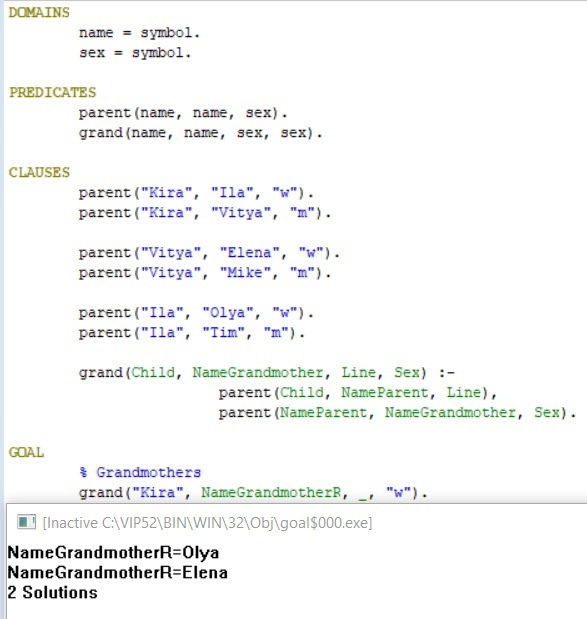
\includegraphics[width=0.9\textwidth]{img/res_lab_16/1.jpg}
        \caption{Поиск всех бабушек}}
    \end{figure}
    
    \begin{figure}[ht!]
        \centering{
            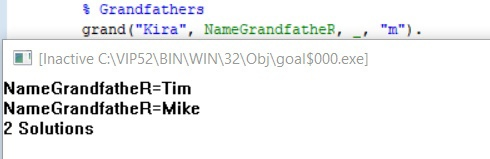
\includegraphics[width=0.9\textwidth]{img/res_lab_16/2.jpg}
            \caption{Поиск дедушек}}
    \end{figure}
    
    \newpage

    \begin{figure}[ht!]
        \centering{
            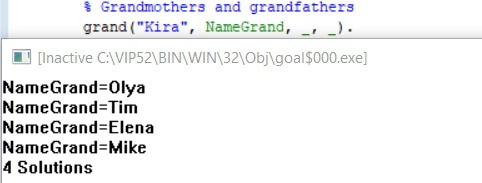
\includegraphics[width=0.9\textwidth]{img/res_lab_16/3.jpg}
            \caption{Поиск бабушек и дедушек}}
    \end{figure}
    
    \begin{figure}[ht!]
        \centering{
            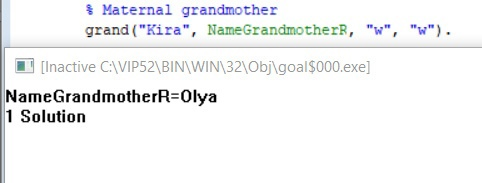
\includegraphics[width=0.9\textwidth]{img/res_lab_16/4.jpg}
            \caption{Поиск бабушек по маминой линии}}
    \end{figure}
    
    \begin{figure}[ht!]
        \centering{
            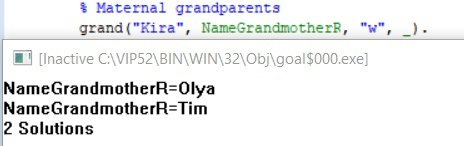
\includegraphics[width=0.9\textwidth]{img/res_lab_16/5.jpg}
            \caption{Поиск бабушек и дедушек по материнской линии}}
    \end{figure}
\end{task}

\newpage

\section*{Практическая часть л.р.17}

\begin{task}
    В одной программе написать правила, позволяющие найти

    \begin{enumerate}
        \item Максимум из двух чисел
        \begin{enumerate}
            \item без использования отсечения,
            \item с использованием отсечения;
        \end{enumerate}
        \item Максимум из трех чисел
        \begin{enumerate}
            \item без использования отсечения,
            \item с использованием отсечения;
        \end{enumerate}
    \end{enumerate}

    \begin{lstlisting}[language=Prolog]
DOMAINS 
    number = integer

PREDICATES
    maximumTwo(number, number, number).
    maximumTwo2(number, number, number).

    maximumThree(number, number, number, number).
    maximumThree2(number, number, number, number).
    
CLAUSES
    maximumTwo(A, B, A) :- A >= B.
    maximumTwo(A, B, B) :- A < B.
    
    maximumTwo2(A, B, A) :- A >= B, !.
    maximumTwo2(_, B, B).
    
    maximumThree(A, B, C, A) :- A >= B, A >= C.
    maximumThree(_, B, C, Res) :- maximumTwo(B, C, Res).
    
    maximumThree2(A, B, C, A) :- A >= B, A >= C, !.
    maximumThree2(_, B, C, Res) :- maximumTwo(B, C, Res). 
    
    
GOAL
    maximumThree(3, 3, 3, Result).       
    \end{lstlisting}

    \begin{figure}[ht!]
    \centering{
        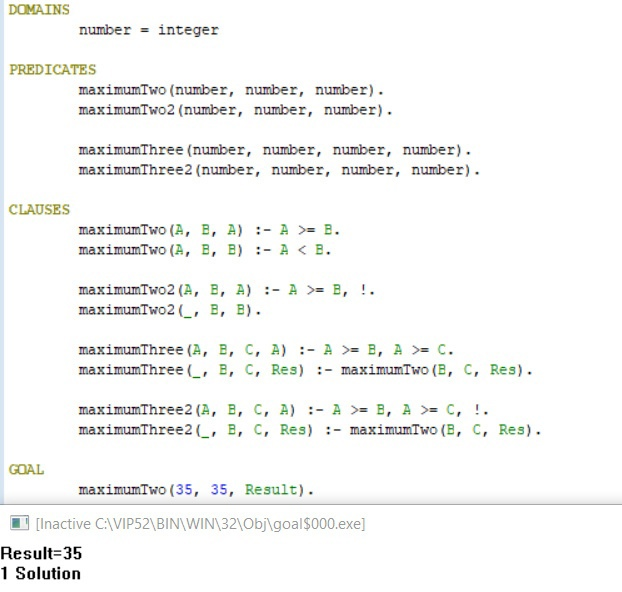
\includegraphics[width=0.9\textwidth]{img/res_lab_17/1.jpg}
        \caption{Максимум из двух чисел}}
    \end{figure}
    
    \begin{figure}[ht!]
        \centering{
            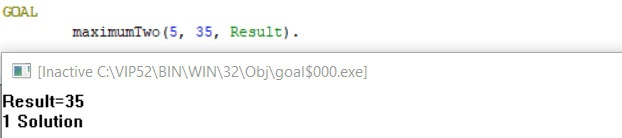
\includegraphics[width=0.9\textwidth]{img/res_lab_17/2.jpg}
            \caption{Максимум из двух чисел}}
    \end{figure}
    
    \begin{figure}[ht!]
        \centering{
            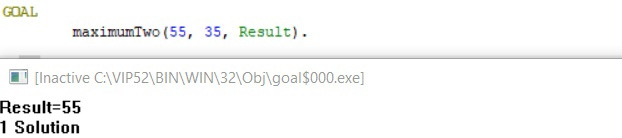
\includegraphics[width=0.9\textwidth]{img/res_lab_17/3.jpg}
            \caption{Максимум из двух чисел}}
    \end{figure}
    
    %  с использованием отсечения
    \begin{figure}[ht!]
        \centering{
            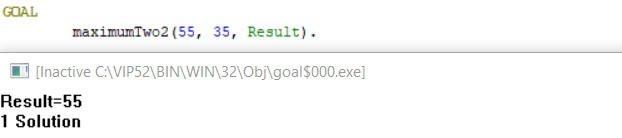
\includegraphics[width=0.9\textwidth]{img/res_lab_17/4.jpg}
            \caption{Максимум из двух чисел с использованием отсечения}}
    \end{figure}
    
    \begin{figure}[ht!]
        \centering{
            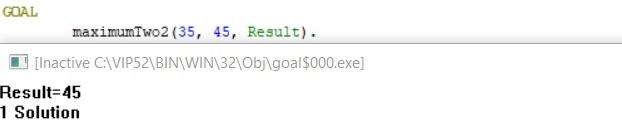
\includegraphics[width=0.9\textwidth]{img/res_lab_17/5.jpg}
            \caption{Максимум из двух чисел с использованием отсечения}}
    \end{figure}

    \begin{figure}[ht!]
        \centering{
            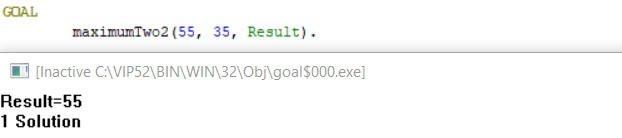
\includegraphics[width=0.9\textwidth]{img/res_lab_17/6.jpg}
            \caption{Максимум из двух чисел с использованием отсечения}}
    \end{figure}

    % Three
    \begin{figure}[ht!]
        \centering{
            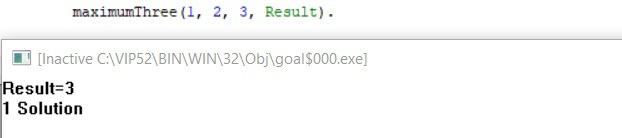
\includegraphics[width=0.9\textwidth]{img/res_lab_17/three/1.jpg}
            \caption{Максимум из трех чисел}}
    \end{figure}
    
    \begin{figure}[ht!]
        \centering{
            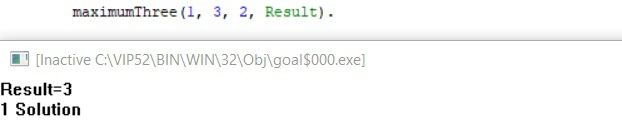
\includegraphics[width=0.9\textwidth]{img/res_lab_17/three/2.jpg}
            \caption{Максимум из трех чисел}}
    \end{figure}
    
    \begin{figure}[ht!]
        \centering{
            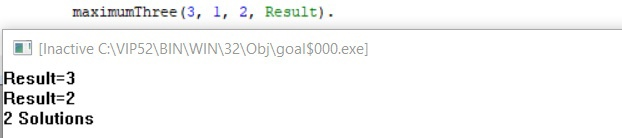
\includegraphics[width=0.9\textwidth]{img/res_lab_17/three/3.jpg}
            \caption{Максимум из трех чисел}}
    \end{figure}

    \begin{figure}[ht!]
        \centering{
            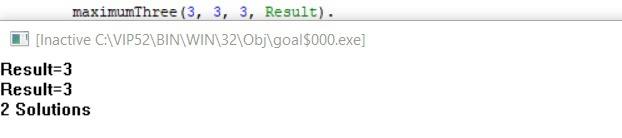
\includegraphics[width=0.9\textwidth]{img/res_lab_17/three/4.jpg}
            \caption{Максимум из трех чисел}}
    \end{figure}


    %  с использованием отсечения
    \begin{figure}[ht!]
        \centering{
            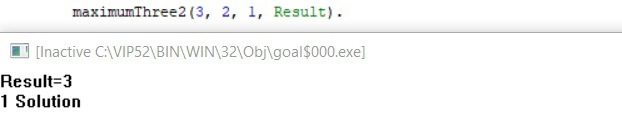
\includegraphics[width=0.9\textwidth]{img/res_lab_17/three/5.jpg}
            \caption{Максимум из трех чисел с использованием отсечения}}
    \end{figure}
    
    \begin{figure}[ht!]
        \centering{
            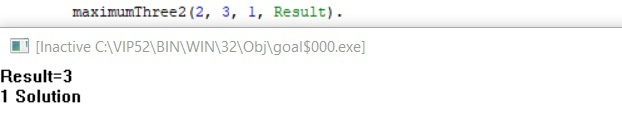
\includegraphics[width=0.9\textwidth]{img/res_lab_17/three/6.jpg}
            \caption{Максимум из трех чисел с использованием отсечения}}
    \end{figure}
    
    \begin{figure}[ht!]
        \centering{
            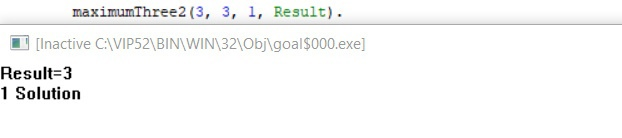
\includegraphics[width=0.9\textwidth]{img/res_lab_17/three/7.jpg}
            \caption{Максимум из трех чисел с использованием отсечения}}
    \end{figure}

    \begin{figure}[ht!]
        \centering{
            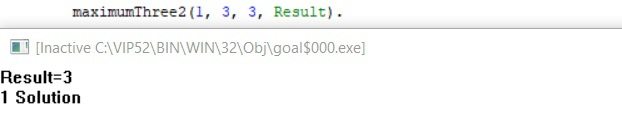
\includegraphics[width=0.9\textwidth]{img/res_lab_17/three/8.jpg}
            \caption{Максимум из трех чисел с использованием отсечения}}
    \end{figure}

    \begin{figure}[ht!]
        \centering{
            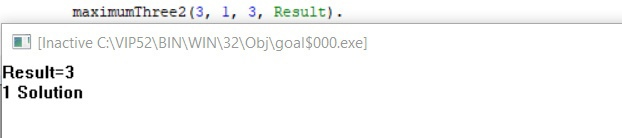
\includegraphics[width=0.9\textwidth]{img/res_lab_17/three/9.jpg}
            \caption{Максимум из трех чисел с использованием отсечения}}
    \end{figure}

    \begin{figure}[ht!]
        \centering{
            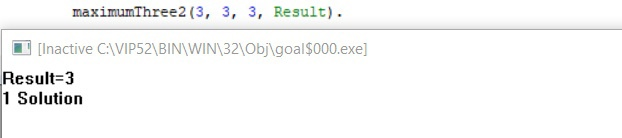
\includegraphics[width=0.9\textwidth]{img/res_lab_17/three/10.jpg}
            \caption{Максимум из трех чисел с использованием отсечения}}
    \end{figure}
\end{task}

\newpage


\end{document}